\documentclass[12pt, letterpaper]{article} 

\usepackage{amsmath, amssymb, amsthm, enumerate, graphicx}

\title{MATH 189 HW 6}
\author{Dani Nguyen}
\date{Winter 2025}

\begin{document}
\maketitle
\graphicspath{ {./} }

\noindent \textbf{Question 1}\
\begin{enumerate}[a.]
    \item 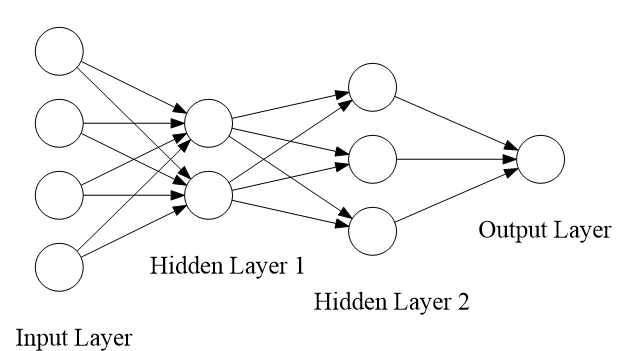
\includegraphics[scale=0.8]{neural_network.png}
    \item 
    \begin{align*}
        f(x) &= \beta_0 + \sum_{k=1}^{3}\beta_kA_k^{(2)} \\
        A_k^{(2)} &= g\left( w_{k0}^{(2)} + \sum_{j=1}^{2}w_{kj}^{(2)} A_j^{(1)} \right) \\
        A_k^{(1)} &= g\left( w_{k0}^{(1)} + \sum_{j=1}^{4}w_{kj}^{(1)} x_j \right)
    \end{align*}
    \item $f(x) = 1 + 2A_1^{(2)} + 3A_2^{(2)} + 4A_3^{(2)}$
    \item $4(2) + 2 + 2(3) + 3 + 3(1) + 1 = 23$ free parameters
\end{enumerate}

\noindent \textbf{Question 2} 
\begin{enumerate}[a.]
    \item 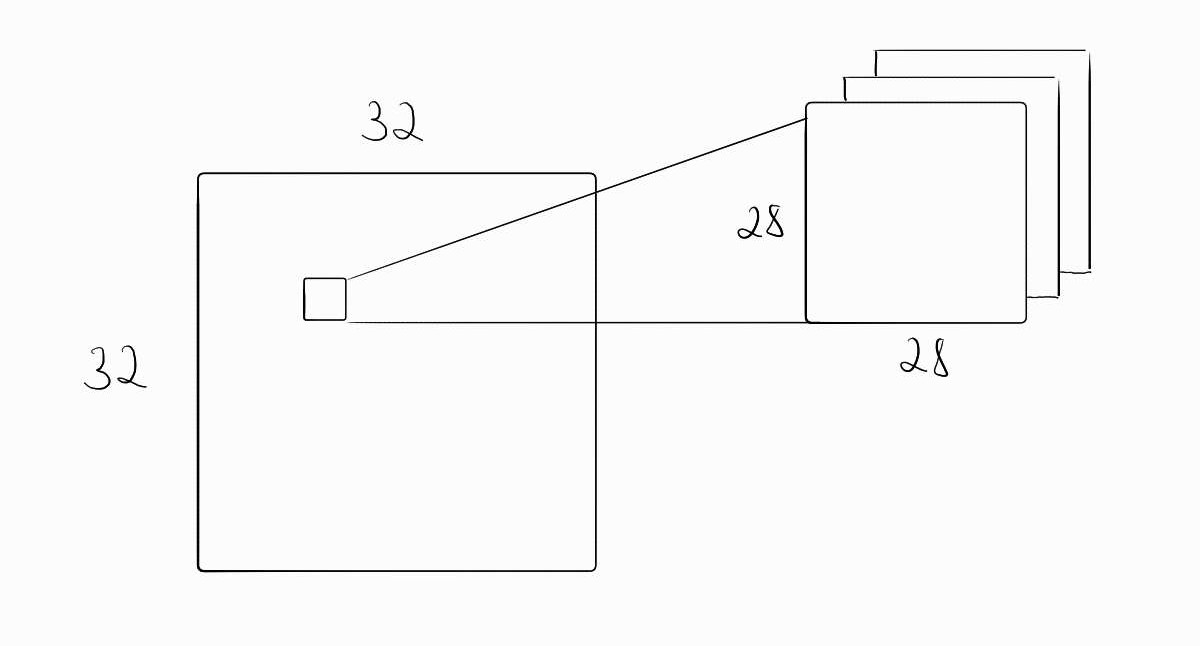
\includegraphics[scale=0.4]{2a.jpg}
    \item There are 3 $5\times 5$ filters each with their own bias terms. Therefore, we 
    have $3(5)(5) + 3 = 78$ parameters.
    \item The constraints are from the convolution filters being $5\times 5$, meaning 
    in the input image, only 25 pixels will impact one pixel on the convolved image, 
    that is one constraint.
    \item If there were no constraints, there would be $(32\times 32+1)\cdot 3(28\times 28) =$ 
    2,410,800 parameters.
\end{enumerate}
\newpage
\noindent \textbf{Question 3}
\begin{enumerate}[a.]
    \item 
\includegraphics[scale=0.8]{3a.png}
    \item \begin{align*}
        \frac{d}{d\beta}R(\beta) = \cos(\beta) + \frac{1}{10}
    \end{align*}
    \item I ran gradient descent with $\rho = 0.1$ for 100 steps, $\beta_{100} = 4.612$ \\
    With $\rho = 1.4$, $\beta_{100} = 4.612$ \\
    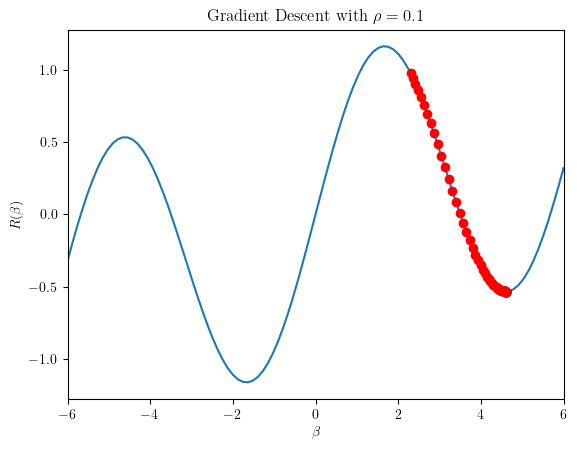
\includegraphics[scale=0.8]{3c.png} \\
    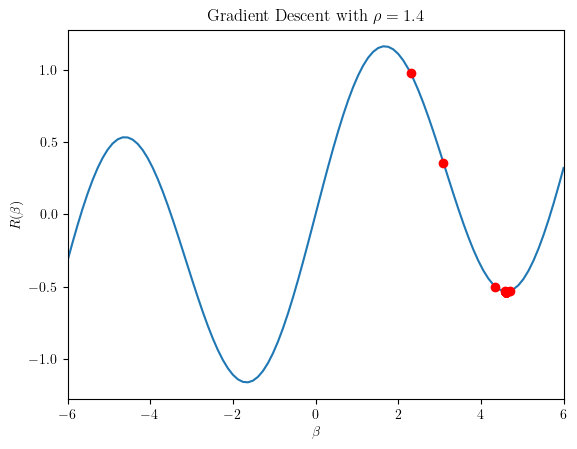
\includegraphics[scale=0.8]{3d.png}
\end{enumerate}

\newpage
\noindent \textbf{Question 4} \\
Skipped


\end{document}